\section{Introduction}\label{intro}

In the current web service age, the deployment of services in off premises is more easy task. The users not even need to estimate their server specifications during the SLA negotiation. This can be possible by the concept of serverless application or Function as a Service (FaaS) \cite{Wang_usenix_2018}. Popular cloud providers such as Amazon, Microsoft, and Google already introduced their serverless solutions as AWS Lamda (https://aws.amazon.com/lambda/), Azure Function (https://azure.microsoft.com/en-in/solutions/serverless/), and Google Cloud Function (https://cloud.google.com/functions/) respectively. Apart from these big players, some new solutions has also started providing the FaaS service \cite{servelless_online_2019}.

\noindent Serverless applications are flexible enough to focus on user's core product and business logic instead of responsibilities like operating system (OS) access control, OS patching, provisioning, right-sizing, scaling, and availability \cite{Lloyd_2018}. By building your application on a serverless platform, the platform manages these responsibilities for you. These new concepts are providing the following capabilities:
\begin{itemize}
	\item \textbf{No server management:} Users need not to provision or maintain any servers. There is no software or runtime to install, maintain, or administer.
	\item \textbf{Flexible scaling:} Users can scale their application automatically or by adjusting its capacity through toggling the units of consumption (for example, throughput, memory etc.) rather than units of individual servers.
	\item \textbf{High availability:} Serverless applications have built-in availability and fault tolerance. Useres not need to architect for these capabilities because the services running the application provide them by default.
	\item \textbf{No idle capacity:} Users need not to pay for idle capacity. There is no need to pre-provision or over-provision capacity for things like compute and storage. There is no charge when your code is not running.
\end{itemize}

%\begin{figure}[!ht]
%	\centering
%	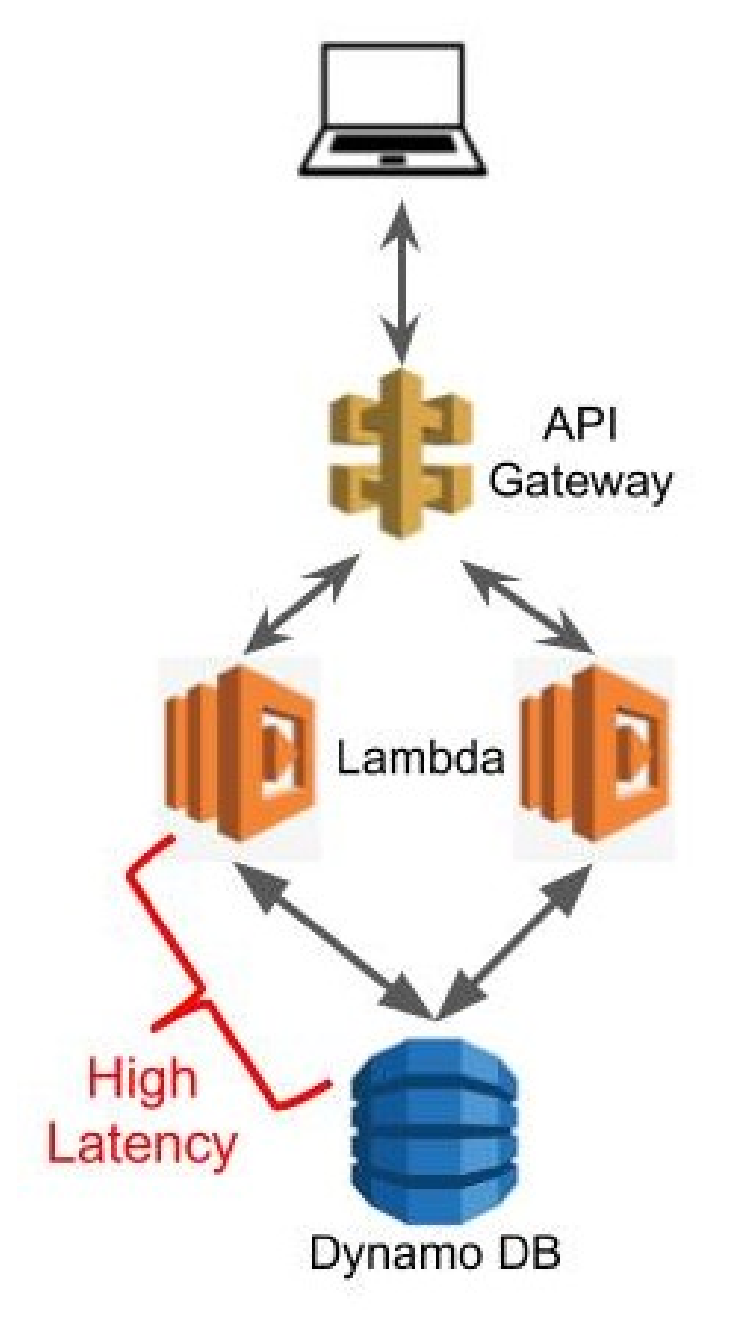
\includegraphics[width=0.5\linewidth, height=0.8\columnwidth]{image/serverless_arch.eps}
%	\caption{Serverless Architecture}\label{fig:serverless_arch}
%\end{figure} 

%\subsection{Some popular serverless usecasess and their archtechture:}
Currently, most of the technology adopters are startups who seek for a possibility to scale painlessly and to lower the entrance barrier. Serverless is also a perfect approach for applications that do not run continuously but rather have quiet periods and peaks of traffic. This concept can be useful for a wide range of applications, from a simple database (DB) application to complex data analytics pipeline applications \cite{Bhattacharjee_USENIX_2019}.
%\begin{enumerate}
%	\item \textbf{Simple DB appliacation:} For any small scale application such as iteractive web site, ERP solutions etc. Serverless is a good candidate to opt as a deployment technology. Figure \ref{fig:simpleDB_serverless} illustrate a simple DB application.
%	
%	\item \textbf{Data analytics pipeline:}
%	\cite{Bhattacharjee_USENIX_2019}.
%\end{enumerate}
% 

%Related work
In the literature, a few recent works have significantly explored serverless computing from different perspectives. In \cite{Akkus_Sand_Usenix_2018}, a new serverless computing system that provides lower latency, better resource efficiency and more elasticity than existing serverless platforms is discussed. To achieve these properties, authores have introduced a model SAND, based on application-level sandboxing and an hierarchical message bus. Here, the design and implementation of SAND, as well as experience in building and deploying serverless applications on it are presented. In \cite{Oakes_USENIX_2018}, the author has analyzed Linux container primitives, identifying scalability bottlenecks related to storage and network isolation where there is a container system optimized for serverless workloads. Based on these findings, they have implemented SOCK, a container system optimized for serverless workloads model. They have identified container initialization and package dependencies as common causes of slow Lambda startup. In \cite{Hong_USENIX_2018}, author has advocated for taking a serverless approach by proposing six serverless design patterns to build security services in the cloud. For each design pattern, they describe the key advantages and present applications and services utilizing the pattern. Using the proposed patterns as building blocks, they have introduced a threat intelligence platform that collects logs from various sources,  alerts malicious activities, and takes actions against such behaviors.

%%\cite{Ishakian_2018}.

Though advantageous in focusing on the user's business logic rather than the platform management, serverless architectures has latency related issues as it is stateless and need to communicate with data source, other serverless functions. In this paper, we analyze this latency of serving requests for different serverless architectures. First, we take the simplest use case of a database application and compare the performance with the traditional VM based approach. Next, we analyze a more complex data pipeline involving multiple functions and observe how it impacts the overall latency of the service. Then, we propose some simple caching strategies to improve the response times. Finally, we discuss their pitfalls.

%Our contributions include:
%(1) Showing database access in AWS lambda function is 80 times more expensive than using traditional VMs.
%(2) Using in memory key value stores like Redis can significantly reduce the latency of database access.
%(3) The lambda containers can cache data for faster access, and it is persisted till a cold start is hit. However there are some challenges as discussed.
%(4) Cascading serverless functions incurs a very big latency penalty.
%(5) Analyze Geo distributed serverless architectures